\documentclass[oneside,
  digital, %% This option enables the default options for the
           %% digital version of a document. Replace with `printed`
           %% to enable the default options for the printed version
           %% of a document.
  table,   %% Causes the coloring of tables. Replace with `notable`
           %% to restore plain tables.
  nolof,     %% Prints the List of Figures. Replace with `nolof` to
           %% hide the List of Figures.
  nolot,     %% Prints the List of Tables. Replace with `nolot` to
           %% hide the List of Tables.
  %% More options are listed in the user guide at
  %% <http://mirrors.ctan.org/macros/latex/contrib/fithesis/guide/mu/fi.pdf>.
]{fithesis3}
%% The following section sets up the locales used in the thesis.
\usepackage[resetfonts]{cmap} %% We need to load the T2A font encoding
\usepackage[T1,T2A]{fontenc}  %% to use the Cyrillic fonts with Russian texts.
\usepackage[
  main=english, %% By using `czech` or `slovak` as the main locale
                %% instead of `english`, you can typeset the thesis
                %% in either Czech or Slovak, respectively.
  german, russian, czech, slovak %% The additional keys allow
]{babel}        %% foreign texts to be typeset as follows:
%%
%%   \begin{otherlanguage}{german}  ... \end{otherlanguage}
%%   \begin{otherlanguage}{russian} ... \end{otherlanguage}
%%   \begin{otherlanguage}{czech}   ... \end{otherlanguage}
%%   \begin{otherlanguage}{slovak}  ... \end{otherlanguage}
%%
%% For non-Latin scripts, it may be necessary to load additional
%% fonts:
\usepackage{paratype}
\def\textrussian#1{{\usefont{T2A}{PTSerif-TLF}{m}{rm}#1}}
%%
%% The following section sets up the metadata of the thesis.
\thesissetup{
    university    = mu,
    faculty       = fi,
    type          = mgr,
    author        = Martin Štefanko,
    gender        = m,
    advisor       = {Bruno Rossi, PhD},
    title         = {Use of Transactions within a Reactive Microservices Environment},
    TeXtitle      = {Use of Transactions within a Reactive Microservices Environment},
    keywords      = {transactions, Narayana, JTA, reactive, microservices, asynchronous, saga, compensating transactions},
    TeXkeywords   = {transactions, Narayana, JTA, reactive, microservices, asynchronous, saga, compensating transactions},
}
\thesislong{abstract}{
abstract
}
\thesislong{thanks}{
   thanks
}
%% The following section sets up the bibliography.
\usepackage{booktabs}

\usepackage{makeidx}      %% The `makeidx` package contains
\makeindex                %% helper commands for index typesetting.
%% These additional packages are used within the document:
\usepackage{paralist}
\usepackage{amsmath}
\usepackage{amsthm}
\usepackage{amsfonts}
\usepackage{url}
\usepackage{menukeys}
\usepackage{minted}
\usepackage{needspace}

\newcommand{\newlinepar}[1]{\paragraph{#1}\needspace{4\baselineskip}\mbox{}\\}


\begin{document}
\chapter{Introduction}

\clearpage
\chapter{Transaction concepts}

This chapter introduces the basic notions of transactions, their properties and common problems of their management across multiple nodes in the distributed systems. 

\section{Transaction}

A transaction is an unit of processing that provides all-or-nothing property to the work that is conducted within its scope, also ensuring that shared resources are protected from multiple users \cite{java_tran_processing}. It represents an unified and inseparable sequence of operations that are either all provided or none of them take effect. 

From the application point of view there exist several transaction models in which the transactions can be executed. The applicable models in the transaction management are local, programmatic and declarative transactions. All three models will be described in detail in the following section.

The transaction can end in two forms: it can be either \textit{commited} or \textit{aborted}. The commit determines the successful outcome - all operations within the transaction have been performed and their results are permanently stored in a durable storage. The abort means that all performed operations have been undone and the system is in the same state as if the transaction have not been started.

Generally the achieving of above features may differ. The most common pattern for the transaction processing is a two phase commit protocol with the ACID transactions. Other approaches are based on the relaxation of the one or more of ACID properties to adjust to the real world environments.

\section{ACID properties}

A transaction can be viewed as a group of business logic statements with certain shared properties \cite{nar_wf}. Generally considered properties are one or more of atomicity, consistency, isolation and durability. These four properties are often referenced as ACID properties \cite{haerder_reuter_1983} and they describe the major points important for the transaction concepts.\footnote{Although, ACID acronym has been associated with transactions since their beginning, Eric Brewer, the inventor of the CAP theorem discussed in the later section, stated in his article from 2012 that it is "more mnemonic than precise".\cite{brewer_2012}}

\subsection{Atomicity}

The transaction consists of a sequence of operations performed on different resources or by different participants. Atomicity means that all operations in the transaction are performed as if they were a single operation. When the transaction commits successfully, all of its participants are also required to perform a valid commit. Conversely, if the transaction fails and is aborted, all performed operations and effects have to be undone. This defines a possibility to abort at any point so that all changes done by the transaction will be reverted to the state present before the transaction started.

The atomicity is commonly achieved by the usage of consensus multi-phase protocols. Standardized protocol is the two phase commit protocol which is used by the majority of modern transaction systems. This protocol, as well as other communication patterns, will be discussed in the later section. 

\subsection{Consistency}

The word consistency refers to restrictions placed on data changes that may happen only in allowed ways. When the data is persisted, it must be valid according to all defined rules which meet the application invariants. The consistency property describes that the transaction maintains the consistency of the system and resources that it is being performed on. When the transaction is started on the consistent system, this system must remain consistent when the transaction ends - it moves from one consistent state to another.

Unlike other transactional properties (A, I, D), consistency cannot be realized by the transaction system as it does not hold any semantic knowledge about the resources it manipulates \cite{java_tran_processing}. Therefore, the achievement of this property is the responsibility of the application code.

\subsection{Isolation}

The isolation property takes effect when multiple transactions can be executed concurrently on the same resources. It provides a guarantee that concurrent transactions can not interfere one with another. Therefore each concurrent execution on the shared resource must be equivalent to some serial ordering of contained transactions. This is why the isolation is often also referred to as a serializability.

From the perspective of an external user the isolation property means that the transaction appears as it was executed entirely alone. This means that even if there are multiple transactions in the system executed concurrently, this fact is hidden from the every external view.

As an instinctive extension of the consistency property, the serial execution of the transaction keeps the consistent state. The execution of the transactions in parallel therefore cannot result into inconsistent system.

\newlinepar{Isolation levels}

In practice we distinguish several levels that describe to which extent the isolation guarantees are provided. Levels are distinguished by simplifications of the locking mechanism in exchange for the faster processing. These levels, in decreasing order, are serializable, repeatable read, snapshot isolation, read committed and read uncommitted isolation. The definitions given in this section are based on the talk given be Martin Kleppmannp\cite{isolation_levels}.

\newlinepar{Read uncommitted}

This is the lowest level which does not place any restrictions on the system. This means that it does not require any form of locking mechanisms to be implemented. It allows dirty reads which is that one transaction may read the not yet committed changes of other transaction.

\newlinepar{Read committed}

Read committed level differs from the previous level in that it prohibits dirty reads and dirty writes. The prevention from dirty reads as discussed in previous section means that the transaction is not allowed to read data that has not been committed by different transaction. 

On the other hand, dirty writes mean that the transaction overwrites the uncommitted data. This can be easily described on an example depicted in the figure 2.1. In this execution the resulting data state contains different values for variables (x = B and y = A). However, in any serial execution of transaction the result would be consistent.

\begin{figure}
    \begin{center}
        \includegraphics[height=45mm]{images/dirtyWrite.png}
    \end{center}
    \caption{Dirty writes}
\end{figure}

\newlinepar{Repeatable read and snapshot isolation}

Both of these methods represent the same level of isolation preventing the anomaly called read skew which can appear in read committed.

The read skew is a problem of reading the data values in different points of time in which the whole consistent data state may not be ensured. This means that the transaction may read the data change in later point in time which may invalidate already read information from a previous processing.\footnote{Imagine a bank system with two accounts both with starting balance 500 and a transfer of 100 from account 1 to 2 as a transaction. If an external system reads the balance of the account 2 prior to start of transaction, it will get 500. However, the subsequent read from the account 1 after the transaction has committed would output 400 which would result into inconsistent information.}

Both repeatable read and snapshot isolation prevent read skews. From the user point of view they represent the same isolation level, but they differ in implementation. Repeatable read is based on the locking mechanisms which may be complex to maintain in bigger systems. The snapshot isolation is implemented as multi version concurrency control that allows each transaction to read the data as it was in one point of time -- the snapshot. The database is required to internally keep track of several states and provide each transaction with the snapshot that is appropriate for its time span.

\newlinepar{Serializable}

On top of the repeatable read, the serializable isolation prevents the system from one more race condition known as the write skew. The basic principle of a write skew is a transaction that reads data from the storage and then makes a decision based on this information. However, different transactions may write the result into different parts of the database which means they can not conflict. The problem is that by the time the transaction commits, the premise of the decision may no longer be true and the resulting state may break the integrity constraints of the database.

\subsection{Durability}

This property characterizes that all changes done by the transactions must be persistent, i. e. any state changes performed during the transaction must be preserved in case of any subsequent system failure. How the state is preserved usually depends on the particular implementation of the transaction system. Generally, to achieve this property the use of the persistent storage like a disk drive or a cloud is sufficient. Even if this kind of storage is acceptable, it still can not prevent data loss in the case of more critical catastrophic failures.



\section{Transaction models}

As it was already mentioned at the beginning of this chapter, there exist three types of transactions models available for transaction management that define how the transaction is composed -- local, programmatic and declarative transactions\footnote{some sources (e. g. Spring) distinguish only two types of transaction models -- the local model and  the global model that represents both programmatic and declarative approaches}. This chapter describes each model respectively and examines how it can be applied in applications deployed in the Enterprise Java platform environment.

\subsection{Local transaction model}

The local transaction model derives its name from the fact that transactions are managed by a local resource manager which will be described in the later section. This approach represents the transaction as a connection to the individual resource. Common use-cases for this model include the Java database connectivity (JDBC) or the Java Message Service (JMS) connection providers.

The connection is usually by default configured to commit or rollback the local transaction after each operation, e. g. a database query or sending a message to a queue. In order to control the transaction, it is required to set the boolean flag \texttt{setAutoCommit} on the \texttt{Connection} interface to false. In this case, the transaction needs to be manually committed or rollbacked with the respective methods of the \texttt{Connection} interface.

The major drawback of this model is that local transactions cannot exist concurrently when coordinating multiple resources using an XA\footnote{XA stands for \textit{eXtended Architecture}, and it is described in detail in section \ref{sec:transaction-manager}} global transaction \cite{java_transaction_design_strategies} (e. g. we need to update a database and propagate this information to the JMS topic).

\subsection{Programmatic transaction model}

This approach is based on the Java Transaction API (JTA) transaction service implementation. In this model, the developer handles the complete management of the transaction in the source code.

The JTA specification is a set of interfaces that allows developers to manage transactions. Another similar term associated with Enterprise transactions is the Java Transaction Service (JTS). The JTS is a specification for the implementation of the transaction manager which encompasses the JTA specification. It represents a Java mapping of the Common Object Request Broker Architecture Object Transaction Service (CORBA OTS) 1.1 specification. The JTA is required to support both JTS and non-JTS implementations of the transaction management.

Although the JTA specification provides a range of APIs, the only required interface for the utilization of the programmatic transactions is the \texttt{javax.transaction.UserTransaction}. The full interface is available at the appendix \ref{sec:appendix-JTA}. The only concerned methods are \texttt{begin()}, \texttt{commit()}, \texttt{rollback()} and \texttt{getStatus()}. The call to the \texttt{begin()} will start a new transaction and associates it with the current thread. As the Java platform allows only one transaction to be associated with the thread, a call to the \texttt{begin()} method may result into exception in case the transaction has already been started in the current context. The transaction end methods (\texttt{commit()} and \texttt{rollback()}) perform their respective actions and disassociate the transaction with the thread. The \texttt{getStatus()} method returns an integer value representing the status of the current transaction derived from  \texttt{javax.transaction.Status} class (appendix \ref{sec:appendix-JTA}).

The most common problem introduced by the programmatic model is that the developer must ensure that the transaction is always terminated in the method that started the transaction \cite{java_transaction_design_strategies}. This is often the case when  the initiating method ends up with an uncaught exception and for this reason, the transaction needs to be committed or rollbacked before the method returns.

\subsection{Declarative transaction model}

The declarative transaction model is also referred to as the Container-Managed Transactions (CMT). In this model, the supplying, underlying container manages all transactions on the users behalf. This includes starting and the administration of the end phases (either commit or rollback) of transactions. The developer is only required to setup the container with the transaction configuration that declares, for instance, that the transaction should be rollbacked on any exception.

The main concerned interface used for declarative transactions is the \texttt{javax.transaction.TransactionManager}. Although this interface provides  same methods that are present in the \texttt{UserTransaction} interface used in the programmatic model, users are strongly encouraged to use it only in CMT. In addition to the \texttt{UserTransaction}, it introduces two methods that manage the transaction suspensions. The \texttt{suspend()} method suspends and  disassociates the transaction with the current thread. It returns an object that represents the identification of the running transaction. This transaction object can be afterwards used as an argument to the \texttt{resume()} method to associate the transaction again with the current thread and continue the transaction execution.

Another essential method that is often associated with the container transactions is the \texttt{setRollbackOnly()}. It declares that the only possible transaction result is to rollback and any consequent actions can not change it.

With the declarative transaction model, the users are required to configure the container with the settings of how individual transactions should be managed. This can be set up through the transaction attribute represented by, for instance, \texttt{TransactionAttributeType}, \texttt{Transactional.TxType} or \texttt{TransactionDefinition} (Spring) classes. The supported values are -- Required, Mandatory, RequiresNew, Supports, NotSupported and Never\footnote{Spring adds one more transaction attribute called Nested which represents a single physical transaction with multiple savepoints that it can roll back to \cite{spring_transaction_management_documentation}}:

\begin{itemize}
    \item \textbf{Required} -- If the transaction context is already present on the invocation, it will be used. Otherwise a new transaction is started. This is the most characteristic attribute and it usually configured as a default value.
    
    \item \textbf{Mandatory} -- Similarly to the Required, mandatory transaction attribute represents that the transaction must be present on the execution. However, it requires that the transaction is already started prior to the invocation. Alternatively, it throws \texttt{TransactionRequiredException} if the transaction context can not be found.
    
    \item \textbf{RequiresNew} -- The container will begin a new transaction on every invocation. If there is already a transaction context present, it is suspended for the duration of the processing of the new transaction. This breaks the atomicity property of the former transaction.
    
    \item \textbf{Supports} -- This attribute represents an invocation that is not required to run under the transaction context. It tells the container to use the transaction context, if it exists before the call, or to execute the operation non-transactionally if the transaction is not present.
    
    \item \textbf{NotSupported} -- The method will not be executed within the transaction context. If the transaction exists prior to the invocation, it is suspended and the method is invoked. In other case, the method is immediately started without the initiation of a new transaction.
    
    \item \textbf{Never} -- The container is forbidden to invoke the method if there is a transaction context present. In contrast with the NotSupported attribute which only suspends former transaction, this attribute will throw a runtime exception when the transaction is present before the invocation.
\end{itemize}



\section{Distributed transactions}

A distributed transaction is the transaction performed in a distributed system.  
The distributed system consists of a number of independent devices connected through a communication network. Such systems are liable to the frequent failures of individual participants or communication channels between them. 

The transaction manager can be implemented as a separate service or being placed with some participant or the client. \textbf{TODO}

\section{Transaction manager}
\label{sec:transaction-manager}

Every transaction is associated with a transaction coordinator or transaction manager which is responsible for the control and supervision of the participants performing individual operations. It is a component liable for coordinating transactions in the sequential or parallel execution across one or more resources. It provides proper and complete execution and it administers the comprehensive result of the transaction.  Applications are commonly required only to contact the transaction manager about the start of the transaction.

The main responsibilities of transaction manager are starting and ending (commit or abort) of the transaction, management of the transaction context, supervision of transactions scoped across multiple resources and the recovery from failure.

\subsection{Local transaction manager}

A local transaction manager or a resource manager is responsible for the coordination of transactions concerning only a single resource. Because of its scope it is often build in directly to the resource. The span of the resource is defined by its managing platform. 

The resource manager is required to provide a support for the participation in the global transactions that span over several resources. This means that it is effectively capable to handle complete transaction processing to the different transaction manager.

\subsection{XA resource}

\section{Failure handling}





CA CP theorem - CAP



\clearpage
\chapter{Microservices architecture pattern}

This chapter introduces the concept of microservices and it focuses on why modern, elastic and resilient enterprise systems should be designed an implemented according to this pattern. It also provides an updated microservices status overview from my previous work publication \cite{bachelor_thesis}.

\section{Architectural pattern}

Microservices are an architectural pattern which offers an intuitive approach to common problems following a software development. They represent a subset of a Service Oriented Architecture (SOA) \cite{soa} that advocates creating a system from a collection of small, isolated services, each of which owns their data, and is independently isolated, scalable and resilient to failure \cite{reactive_ms_arch}. Instead of the SOA, which builds the applications around the system logical domain, microservices are focused around the application business model. Each microservice represents the separated and independent part of the system that interacts with other components only through predefined communication interfaces\footnote{throughout the rest of this publication we will be using terms \textit{microservice} and \textit{service} interchangeably}.

\subsection{Monolithic architecture}

The effective way of describing why the microservice architecture is emerging as a practical development style, is to begin with the definition of the opposite pattern -- the monolithic architecture. When the application is developed in the monolithic fashion, all of its content is being implemented and deployed as a single archive. Every component, i. e., a unit of software that is independently replaceable and upgradeable \cite{microservices}, is tightly coupled within the application. Because of the easy development of the monolithic software, this approach has been preferred by the majority of edging enterprise applications. However, when the application requires to add a new functionality or to fix a problem, any additional maintenance represents an issue. For instance, even because of the minor change or update in the single component, the scalability, continuous deployment and the general advancement of the whole application can stagnate. 

Monolithic applications present a few advantages -- the development model is often easy to adjust to the application requirements\footnote{the traditional development model represented as the client-server-database or the Model-View-Controller architecture \cite{mvn_architecture}}, the deployment is reduced to single archive (or a small number of archives) and it is easy to horizontally scale by adding more servers behind a shared load balancer. The problems arise when the system becomes large. The monolithic code base is often complex and hard to understand which results into long learning curves \cite{learning_curve} and developer concerns. The automatic deployment and the continuous delivery (CD) of the system also decelerate -- in order to update one component you have to redeploy the entire application \cite{monolithic_arch}. Although, it is still able to scale horizontally, the replicated server instances take up more resources and overload the container with a slower start up speeds. In general, the monolith also represents a commitment to a particular technology (or even its specific version) which makes the system difficult to maintain and also adapt to new emerging technologies.


\subsection{Microservice architecture}

Microservices introduced the application separation into the self-maintained units – services \cite{intro_to_microservices}. The service is a single scalable and deployable unit, which is not dependent on any context. This means that services may be deployed and scaled independently of each other, and may employ different middleware   stacks for their implementation \cite{ms_arch_ecommerce}. 

The important attribute of the microservices system is a service isolation. Each microservice is responsible for the management of its own resources and it is prohibited to directly access resources of any other service. This means that each data request must be processed by the operating microservice which is allowed to accordingly control the data access and computation requirements. Services often correspond to components in the monolithic architecture.

Microservices further extends the Law of Demeter which intents to organize and reduce dependencies between classes \cite{law_of_demeter}. As the service presumably requires to communicate with other services in order to provide system functionality, this law naturally applies to minimize such coupling among microservices on the distributed component level. 

Another standard object-oriented rule that also applies in the microservices environment is the Single Responsibility Principle (SRP) as defined by Robert C. Martin -- a class should have only one reason to change \cite{agile_ppp_c}. There is a common misconception associated with the microservice architecture -- the word \textit{micro} should conform to the service size. Although, this statement is true to some extent (there is no point in creating the microservice of the same size  as the monolith), the \textit{micro} should more resemble a scope of the service responsibility. This concept also corresponds to the Unix philosophy: Make each program do one thing well \cite{unix_time_sharing_foreword}.

The separation and loose coupling of microservices provide an ability to deploy each individual service to the production environment autonomously, not affecting other applications or services. This allows isolated teams to develop, maintain and upgrade services independently and to form these teams around the system problem domains. 

As microservices represent a stateful entities, to achieve data isolation each service exposes an application programming interface (API) through which it is exclusively able to provide functionality to other services. These APIs are often technology-agnostic to ensure that the technology choices are not constrained \cite{building_ms}. Instead of in-process calls employed in the monolithic architecture, applications based on the microservices style utilize services by remote procedure calls which are often asynchronous. This form of segregation also facilitates the system failure recovery or resilience as each particular microservice breakdown is less prone to influence the rest of the system.

\section{Principles of microservices}

This section describes the microservices architecture from the perspective of the business use cases and the solution architecture. It is based on the work of Sam Newman \cite{building_ms, principles_of_microservices} in which he proposed to build each microservices system on a set of principles. This principles may differ for various systems (depending of the application and microservices use cases) but in general, they can reduced to these eight principles:

\begin{enumerate}
	
	\item \textbf{Modeled around the business concepts} -- When the  microservices applications, together with the teams that are responsible for their maintenance, correspond to the business domain, they are generally more stable -- the requirements on their functionality do not change frequently. This allows developers to focus on the particular system segment, rather than on some specific technology stack. Additionally, it also permits services to directly reflect the business requirements.
	
	\item \textbf{Adapting a culture of automation} -- Because of the  service motion, failures or the communication distribution through the network, microservices brings additional complexity to the system. When the number of services increases, the maintenance, administration and deployment can became unmanageable. The automation then presents an essential part of the service life cycle. The practices as the automated service testing, the employment of the continuous delivery or the unification of the deployment strategy over services, allow enterprise systems to scale more efficiently and speed up the mechanism of the service coordination.
	
	\item \textbf{Hiding the internal implementation details} -- Every microservice generally needs to interact with other services or external systems to provide its functionality to the rest of the system. In order to keep the option of independent development, it is essential that each service hides its implementation details. This can be achieved through the motion of bounded contexts as defined for the Domain-Driven design (DDD) \cite{ddd}. The bounded context delimits the applicability of a particular model so that team members have a clear and shared understanding of what has to be consistent and how it relates to other contexts. The context is separated by an explicit interface represented as an API which allows teams to specify which utilities of the service can be shared and which must be hidden. Every request for the service data must be subsequently processed through this public interface.
	
	\item \textbf{Decentralizating all things} -- Microservice architecture is build around the idea of self-sustaining development which means that services are maintained autonomously. This allows to delegate decision making and authority to the team that is accountable for the service maintenance. The team is then able to take full ownership of the service which with the support of the independent deployment mechanism results into the convenient development, testing and life-cycle management. This principle accentuates that relevant business logic should be kept in services themselves and the communication between them must be as simple as possible. This permits to design systems in a way that adheres to the Conway's law  stated in 1967:
    
    \begin{displayquote}
       Any organization that designs a system (defined broadly) will produce a design whose structure is a copy of the organization's communication structure. \cite{conways_law}
    \end{displayquote}

    This principle also affect the system architecture and design. The purpose is to avoid approaches like enterprise service bus (ESB) or other orchestration systems, which can lead to centralization of business logic \cite{building_ms}. In general, architectures build on the choreography patterns rather than orchestration are preferred. The comparison of these two approaches has been investigated in many research works \cite{chor_and_orch, service_oriented_design, realtime_ws_orch}.
	
	\item \textbf{Independent deployments} -- This is the most important principle of the mircroservices architecture. When the service is being deployed, it should be the requirement that it cannot influence the lifespan of any other service. To achieve this, various techniques like consumer-driven contracts or co-existing endpoints can be used. Consumer-driven contracts make services to state their explicit expectations. These requirements are supported by the provided test suite for individual parts of the domain and they are run with each Continuous integration (CI) build. Co-existing endpoints model accommodates consumers to service changes over time. The idea is to make new endpoint which can process updated client requests while the former endpoint still functions for a limited lifespan. This includes techniques as blue/green releases \cite{blue_green} or canary deployments \cite{canary_deploy}. Customers can utilize both endpoints depending on the version their applications require which allows them to decide when to upgrade. Once the previous endpoint is no longer in use, it can be safely removed.
	
	\item \textbf{Customer first} -- Services exist to be called. It is indispensable to make these calls as simple as possible for the customers. The developers can advatage from any feedback from the clients that use their service. To ease the understanding of the service API, it should be supported by a good documentation provided by API frameworks like Swagger \cite{swagger}. This also includes the service discovery mechanisms to propagate system services and to make the discovery of the service providers more apparent. To combine this information we can use the humane registries \cite{humane_registry} which indicate the human interaction. 
	
	\item \textbf{Failure isolation} -- Even if microservices force distributed development it is not a necessity that the failure of one service cannot influence another. This principle describes the distribution of resources to avoid the single point of failure. As there are many vulnerabilities in applications which can break, there is no precise manual on how to attain this principle.
	
	\item \textbf{High observability} -- Monitoring is an important part of development. As the microservice architecture is distributed it can be complicated to process this information. To make it more accessible aggregation is essential. Storing all logging entries and statistics in one place can highly impact the monitoring process. Another relevant point is to track the service calls as the services typically communicate with other services. By logging this information we can ensure traceability in case of failure.
	
\end{enumerate}

\section{Reactive microservices}

Before the definition of what the reactivity means in distributed microservices environments, it is appropriate to start from the basics of what the reactivity signifies in general terms and how these principles may be applied in software architectures. This section introduces the motion behind the reactive design and why it is suitable for the use in the microservices environment.

By the definition in the Oxford dictionary, the word \textit{reactive} symbolizes an exposure of a response to a stimulus or an action in response to a situation rather than creating or controlling it. This definition naturally translates to software systems. However, the interpretation of what the stimuli is in software applications may differ. It might be, for instance, events, messages, requests or failures. The important common property of these impulses is that the development model cannot be implemented in a way to control them. This motions differ from the traditional style of programming models in which the program functioned as a sequence of commands that were always executed in the predefined order and in the maintained, controlled state.

In software systems we distinguish two distinct classes of reactive concerns -- reactive systems and the reactive programming. 

\subsection{Reactive systems}

Reactive systems are an architectural style that focuses on the responsiveness. By the definition provided in the Reactive Manifesto \cite{reactive_manifesto}, reactive systems are also resilient, elastic and message driven which makes them more flexible, loosely-coupled and scalable. Generally, this model provides a straightforward programming interactions and simplified dependency management that is required in modern applications. The following enumeration explains these essential properties in detail:

\begin{itemize}
    \item \textbf{Responsiveness} is the most important characteristic of reactive systems. It provides a guarantee of a timely response to normal user requests, as well as the rapid failure detection. Reactive systems are expected to establish a sufficient upper bound placed on the system response times to institute an end user assurance in the system usage.
    
    \item \textbf{Resilience} covers the responsiveness of the system in the case of the system failure. The manifesto states that the system is not resilient, if it becomes unresponsive after any failure. Resilience can be achieved by, e.g., replication, isolation, delegation and loose-coupling. This ensures that the failure in one part of the system cannot effect the system as whole which shadows the component clients from any form of the failure handling.
    
    \item \textbf{Elasticity} involves the system responsiveness in the case of alternating load. Reactive system is expected to be able to dynamically adjust and scale system resources according to the request traffic. Elasticity also implies that the system must be able to actively replicate and regulate its components and distribute user inputs among them by the scalable, predictive (and possibly reactive) algorithms.
    
    \item \textbf{Message driven} elaborates on the asynchronous message exchange between the system components that promotes the loose coupling, isolation and location transparency. Explicit message utilization has many advantages, e.g., flow control, load management or monitoring and engagement of the back pressure. The location transparency, based on virtual addresses, decouples individual components. It may also provide a failure management mechanism, in which case the service cannot distinguish between the communication with a single component or a cluster. Additionally, the asynchronicity allows the system to utilize resources in a non blocking way, only when they are required for the request processing. 
\end{itemize}

\subsection{Reactive programming}

Reactive programming is a development model focusing on the observation of data streams, reacting on changes, and propagating them \cite{building_reactive_ms_in_java}. In the rest of this section, we will be referencing these data streams in the Reactive Extensions methodology as \textit{observables}. An observable is an object that contains dynamically versatile data that represent state which may be of interest to other object. In order to consume the data emitted by an observarble, the interested object must \textit{subscribe} to it.

In practice, reactive programming distinguishes three kinds of observable objects -- observable data streams, singles and completables. Observable, as a stream of data, represents an asynchronous reaction. It provides three handlers, namely, for the data result, error handling and the end of the data stream. The single is a special type of observable that depicts the stream of one value. It is associated with an execution of asynchronous operation which provides data and error callback handlers. The completable observable symbolizes the stream without any value. It contrast with the single, it do not return a data value. For this reason, the completable should be configured with the completion and error handlers.

The observable stream can be of two types -- a cold or hot observable. The cold observables are lazy loaded. This means that the data stream do not process any tasks until somebody starts observing it. It represents an asynchronous action that is invoked only when there is a consumer interested in the result. When an object subscribes to a cold observable, it receives all data objects contained in the stream which allows them to be shared. Conversely, the hot observable data stream is active before the consumer subscriptions. When the consumer subscribes to the hot observable, it will receive all data values from the stream that are emitted after the subscription. Both cold and hot observables require the user subscription to receive the data values from the streams. If the consumer does not subscribe to an observable stream, the data is lost.

The most important concept of reactive programs is the asynchronicity. On the contrary from the traditional program invocations, this processing model is based upon notifications that are emitted when the data stream produces a value. Each asynchronous operation happens independently of the main program flow which introduces several new aspects that needs to considered for this kind of programming paradigm. These aspects can be summarized in three simple rules: avoid side effects\footnote{The side effect is any interaction of the function with the remainder of the program in other way than through its arguments or its return value}, avoid using too many threads and never block.

One of the most popular implementations of the reactive programming principles in modern systems is the Reactive eXtension (RX). It represents a library for asynchronous and event-based programs by using observable sequences \cite{rxJava}. These extensions combine the observer and iterator patterns with a range of functional idioms to allow developers to easily adapt reactive methods. Reactive extensions provide a broad range of implementations for various programming languages as, for instance, Java (RxJava), C\# (Rx.NET) or Kotlin (RxKotlin). 

To conclude, it is important to remember that reactive programming does not build a reactive system \cite{5thingsAboutRP_RHDev}. It only provides a development model that can be used for asynchronous processing, a task based concurrency model or the non-blocking I/O\footnote{Input/Ouput} that may be employed with other reactive principles to create responsive and reliable distributed systems as defined in the Reactive Manifesto.


\clearpage
\chapter{Communication patterns}

\section{Consensus protocols}

\subsection{2PC}

\subsection{3PC raft paxos}

\section{Event based protocols}

Eventual consistency

\subsection{CQRS}

\clearpage
\chapter{Saga pattern}

A saga, as described in the original publication \cite{sagas_publ} from 1987, is a long lived transaction that can be written as a sequence of transactions that can be interleaved with other transactions. Each operation that is a part of the saga represents an unit of work that can be undone by the compensation action. The saga guarantees that either all operations complete successfully, or the corresponding compensation actions are run for all executed operations to cancel the partial processing (\ref{fig:tripExample}).

\begin{figure}
    \begin{center}
        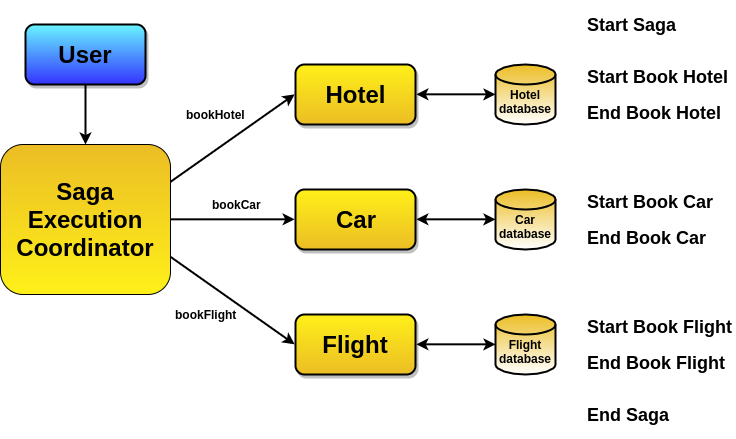
\includegraphics[height=60mm]{images/tripExample.png}
    \end{center}
    \caption{Example saga execution}
    \label{fig:tripExample}
\end{figure}

In contrast to the traditional transaction approach, the Saga pattern relaxes some of the ACID properties (namely atomicity and isolation) to achieve availability and scalability with build-in failure management. In practice, applications are mostly not fully restricted to all of the transaction guarantees, so the saga pattern is emerging as a real alternative to traditional ACID transactions.

In this chapter, we will describe the saga processing as it is defined by the initial publication \cite{sagas_publ}, describe how the activities and compensations works in sagas, how the saga can handle the failure recovery and present several modern frameworks that provide the support for the saga implementation.

\section{Activities}

An activity represents a local transaction that is a part of the saga. Each saga can be split into a sequence of activities in which each individually can be implemented with full ACID guarantees. When the activity completes, all results of the performed work are expected to be persisted in the durable storage. This means that the external observer may see the system in intermediate states of the saga execution, as well as that it may also introduce the system into an inconsistent state between the individual activity invocations.

The ability to commit a local transaction breaks the atomicity property as we no longer endure the atomic unit that the enclosing transaction represents. Furthermore, if distinct sagas may be executed in the system concurrently, the isolation (serializability) property is also violated. Although, intermediate saga states may introduce consistency contraventions, sagas guarantee that the state will become consistent after the saga completes. This principle is called an eventual consistency. It guarantees that even if partial execution may result into the inconsistent state, the system state will get consistent eventually -- there exist a point in future in which the system is consistent.

As the definition in the original paper by Garcia-Molina and Salem \cite{sagas_publ} allows local transactions to interleave, it prohibits any form of dependencies between them. This would imply that the participant cannot depend on results committed by any previous transaction in the saga sequence. However, in modern systems the sequential execution of local transactions is possible to implement in expense of an utilization of a single saga coordinator process throughout the entire sequential execution of this sequence. 

\section{Compensations}

Each activity in a saga needs to have an associated compensation transaction. The purpose of the compensating transaction is to semantically undo the work performed by the original transaction. This is not necessarily the contradictory action that puts the system into the same state as it was present before the activity began or generally the saga started. 

Imagine that the activity consists of the sending of an email. The saga compensation transaction cannot directly undo the email consignment. Instead it would send another email to the same destination which could explain why the previous action did fail. In this case, we can see that the system is in the state where it has two additional emails being send. However, the comprising system state is expected to be semantically consistent as both transaction and compensation have been defined by the participant. Therefore, the consistency guarantees must be ensured by individual participants at the activity level.

The compensating actions for the individual activities are expected to be idempotent. The main reason for this requirement is the saga failure and recovery management which in detail described in section \ref{sec:recovery-modes}.

It is important to keep in mind that even the compensating transactions may fail. There are several options of how the saga management system can handle such situations. The first option is to retry the compensating transaction again, but as the reason of the failure may still be valid, the system can get caught in an infinite retry loop. Another option is to provide a recovery block -- a separated block of code which would get executed in place of the primary compensation in case of failure. The last option, which is not elegant but it is practical, is the manual intervention. This is possible to implement due to the saga nature -- it does not hold any locks on resources it is being performed on. When the compensation handler is manually repaired, the saga can continue its execution where it has left off.

\section{Saga execution component and transaction log}

The saga execution component (SEC) is a process that is responsible for the saga management. It communicates with the transaction manager which manages activities included in the saga. Both of these components require a transaction log to record their respective interactions\footnote{it is convenient to share the transaction log between both components}. The saga execution component does not require  concurrency control because the saga activities can be interleaved.

The entries that may be written to the transaction log are usually associated with the saga or activity lifecycle. The saga log includes \texttt{start-saga} entry followed by one or more \texttt{start-activity} / \texttt{end-activity} entries and it is finished by the \texttt{end-saga}. Optionally, the transaction system may also provide an ability for users to cancel the saga execution with the \texttt{abort-saga} command. 

Each saga operation is channeled through the saga execution component and it is recorded in to the transaction log before any action may be taken. The transaction log can also contain any parameters associated with the saga execution.

\section{Recovery modes}
\label{sec:recovery-modes}

The saga paper \cite{sagas_publ} distinguishes two options to handle the failure that interrupts the saga. These two supported modes are backward and forward recovery.

\newlinepar{Backward recovery}

A backward recovery mode is the most common way of handling saga failure management as it was described in previous sections. It requires that all activities must define a compensation handler.

When the SEC component receives an \texttt{abort-saga} command in the backward recovery mode, it firstly abort the currently executed activity. Then for every previous activity in the reverse order of the original execution, it calls its respective compensation action. After the invocation of the compensation handler corresponding to the first activity is completed, the saga may end and the system is in semantically consistent state as it was before the saga began.

When the saga management system applies the backward recovery mode, the associated transaction log is also used to recover from the crashes of the saga coordinator. After the recovery, once all activities has been completed (committed or aborted), the saga coordinator determines the status of each saga execution by the investigation of transaction log entries. 

If the log contains only both \texttt{start-activity} and \texttt{end-activity} entries for the activities comprised in the saga,  than the execution is safe to continue with the next activity which has not been started. Another safe state is when the transaction log contains the \texttt{abort-saga} entry. In this case, it calls all compensation handlers for the referenced saga. This is possible due to the fact that all compensating actions are required to be idempotent.

The only unsafe state, that may be introduced after the saga coordinator recovers, is when the transaction log contains the \texttt{start-activity} entry without the corresponding \texttt{end-activity}. In this case, the saga coordinator selects the last successfully executed activity (contained in the transaction log) and invokes the compensation handler for this activity and all activities that have been executed before it.

As in the case of repetitive recovery for the same saga, the saga coordinator may call the corresponding compensation handlers repeatedly, the compensation actions are required to be idempotent. The original paper acknowledges that this constraint may be difficult to implement in some applications which is the reason for the introduction of the forward recovery mode discussed in the following section.

\newlinepar{Forward recovery}

For the use of the forward recovery mode, the transaction management requires that the saga itself is predefined and that the system is able to produce a check point. The check point represents a snapshot of the system state in the particular point in time into which the system can be always restored.

The pure forward recovery mode takes the checkpoint automatically at the beginning of each activity. Furthermore, it also disallows to abort the saga intermediate execution. This effectively eliminates the need to define any compensation actions. If the crash of the SEC occurs, it will abort the last executed activity and restart the saga from the last checkpoint. This approach effectively degrades the saga execution component to a basic persistent transaction executor, therefore loosing most of the saga benefits.

\hfill \break

In addition to modes defined above, it is also possible to combine these two approaches into the backward / forward recovery mode. In this mode, the transaction system takes checkpoints in predefined intervals which may be periodical or based on a different criteria (e. g. the activity complexity). In case of the SEC failure, the system performs the backward recovery to the last defined checkpoint and then continues the saga execution in forward recovery mode.

\section{Distributed sagas}

The notion of sagas can be naturally extended into distributed environments. The Saga pattern is an architectural pattern that focuses on integrity, reliability, and quality, and it pertains to the communication patterns between services \cite{prac_ms}. This allows the saga definition in distributed systems to be redefined as a sequence of requests that are being placed on particular participants invocations. These requests may provide ACID guarantees, but this not restricted and it must ensured by individual participants. Similarly, each participant is also required to expose the idempotent compensating request which can semantically undo the request that is handled by this participant in the saga.

Analogously to the non-distributed systems, the distributed saga management also requires a transaction log which needs to be durable and distributed. The examples of distributed database providers include e.g. Cassandra, RethinkDB or Apache Ignite.

The saga execution coordinator (SEC) is spanned process across the participating services. This process manages and interprets the saga and it persists all processing information into the transaction log. The coordinator does not represent a single point of failure as it is allowed to fail. This is possible because the SEC process does not hold any state data, all of the saga state is held in the distributed log. The general example of the application model employing SEC is available in the figure \ref{fig:SEC}.

\begin{figure}
    \begin{center}
        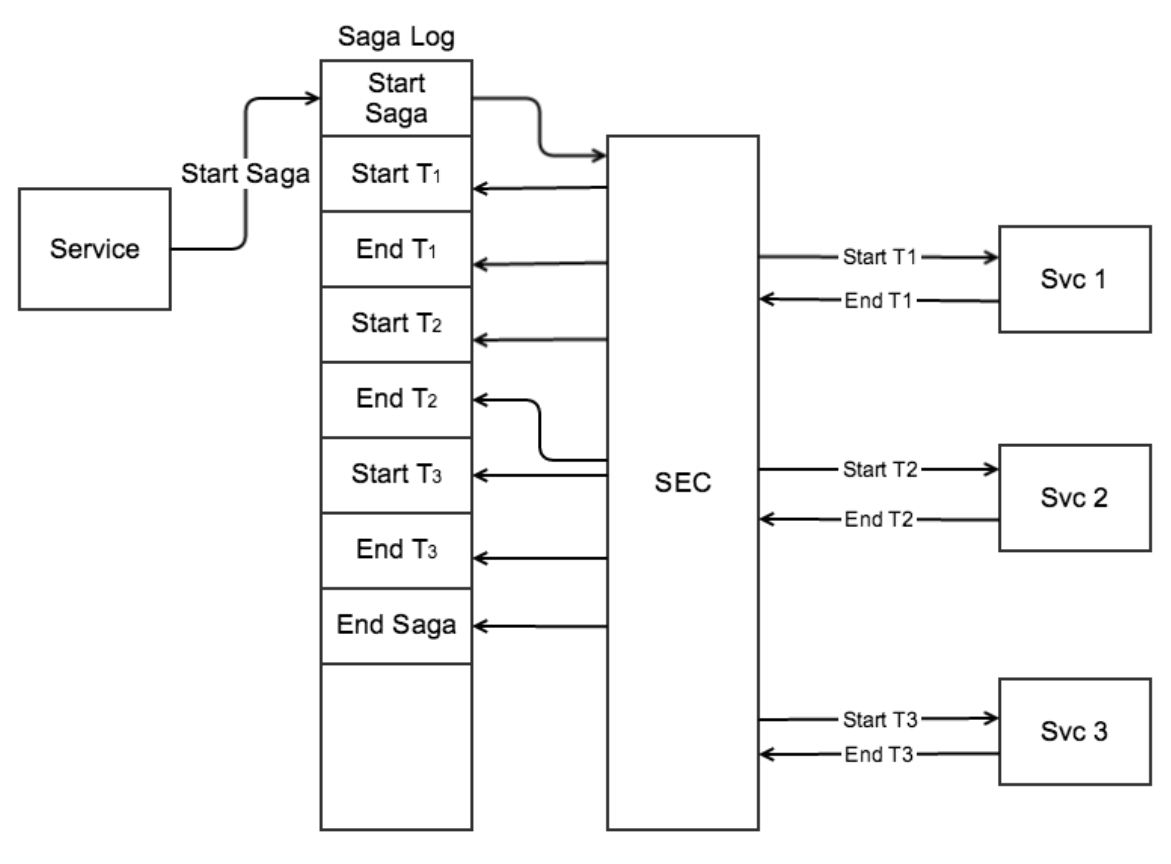
\includegraphics[height=70mm]{images/SEC.png}
    \end{center}
    \caption{Distributed saga example \cite{applying_saga_pattern}}
    \label{fig:SEC}
\end{figure}

As all of the above mentioned components are distributed, the saga management system needs to deal with a number of additional problems that are not present in the localized environment. The main problem is that the saga system is required to deal with network and participant failures that may happen between the remote invocations. There are four locations that can encounter the network failure -- writes for the beginning and end of the request to the transaction log and the request and response calls to the associated participant. This may introduce unnecessary saga aborts\footnote{if the SEC fails after it has written the \texttt{start-request} entry to the transaction log -- the recovery cannot determine whether the failure happened before the request, due to the network failure, or the participant response has been lost}, but generally the approaches from the non-distributed environment still apply.

\section{Current development support}

This section presents the current implementations of the saga pattern available for the enterprise use. The three explored frameworks are Axon \cite{axon_framework}, Eventuate \cite{eventuate.io} and Narayana Long Running Actions (LRA) \cite{narayana_lra}.

\subsection{Axon framework}

Axon is a lightweight Java framework that helps developers build scalable and extensible applications by addressing these concerns directly in the core  architecture \cite{axon_framework}. It is composed on the top of the Command Query Responsibility Segregation (CQRS) pattern which is described in more detail in the Appendix A.

The Axon framework is based upon the event processing including asynchronous message passing and event sourcing. This allows components to be loosely coupled and therefore easily developed in the the microservices manner.

\newlinepar{Saga definition}

As the most of the Axon functionality, the easiest way to define sagas in an application is by the use annotations. The annotation \texttt{@Saga} marks the class as a saga implementation. In Axon sagas are a special type of event listeners. Each object instance of the saga class is responsible for managing a single business transaction. This includes the management of the saga state information, the execution and handling of the transaction (including start and stop) or the performing of the corresponding compensation actions.

All interaction with the saga class happens only by triggering of events. The ordinary event handlers in saga instances are annotated with the annotation \texttt{@SagaEventHandler}. 

To start a saga execution the framework needs to receive the event with the special event handler annotated with \texttt{@StartSaga}. By default, the new instance will be created only if the corresponding saga can be found.

Ending of the saga can be defined in two means -- by the event or by the API call. If the ending event is used, than the conforming event handler needs to be annotated with the \texttt{@EndSaga} annotation. Alternatively, the conditional end of the saga can be signaled by the call to the \texttt{SagaLifecycle.end()} from some method inside the saga class.

As many instances of the saga class may exist at the same time, there is a need to publish events only to the saga for which they are intended. This is done by a definition of association values. The association value is a simple key-value pair where the key is a property present in the event which forms a connection to the saga instance. The \texttt{@SagaEventHandler} annotation contains a custom attribute called the \texttt{associationProperty} which denotes the key property in the incoming event. Axon also allows the definition of additional association values by a call to the \texttt{SagaLifecycle.associateWith(key, value)} and the \texttt{SagaLifecycle.removeAssociationWith(key, value)} inside the saga class.

\subsection{Eventuate.io}

To correctly connect to the Eventuate platform structure, services are required to specify a collection of the application properties. These options define connection and authentication details for Eventuate support services. The Spring Boot application can specify these attributes in an \texttt{application.properties} file or as environment variables.

\subsection{Narayana LRA}

The coordinator is responsible for the LRA starting, progress tracking and either completion or compensation. 


\subsection{Eventuate Tram}

the platform controls the information transfer. The base Eventuate platform builds the communication exchange on top of the event processing. On the other hand, Tram handles the command responses as messages send trough dedicated channels. 
 


\clearpage
\chapter{Saga implementations comparison example}

As a part of the investigation of the each discussed framework from the previous chapter, I created a sample application simulating the saga utilization. The main goal of this quickstart projects is to compare the base attributes of the investigated saga solution frameworks. This includes the comparison of the development model, microservices feasibility, maintainability, scalability, performance and the applicability of the reactive principles within the saga execution. 

The application represents a backend processing for orders with a simple REST\footnote{Representational State Transfer} user interface. Users are also allowed to query persisted information through the defined microservices APIs available in appendix \ref{sec:appendixAPI}.

All examples are based on the microservices pattern. As every framework is suitable for the use in different environments, each example is achieving the same goal through the different portfolio of technologies. The exact mechanisms used is individual projects will be discussed in more detail in their respective sections.

\section{Common scenario}

A user is able to create the order by a REST call to the dedicated endpoint of the \texttt{order-service} microservice. The request must provide a product information JSON\footnote{JavaScript object notation} containing a product id, a commentary and a price. For the simplicity reasons, the order always consists only of the single product. The figure \ref{fig:inputJson} shows the example of the input JSON format for the product data. The complete REST API\footnote{Application programming interface} for each individual example is provided in the Appendix \ref{sec:appendixAPI}.

\begin{figure}
    \begin{center}
        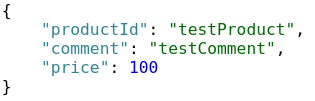
\includegraphics[height=30mm]{images/productInfoJSON.png}
    \end{center}
    \caption{Product Information example JSON}
    \label{fig:inputJson}
\end{figure}

The setup of each example is described in detail in their respective repositories included in the Appendex B. Generally, each service is a standalone Java application that must run in a separated terminal instance by default located on the local computer address (localhost). Except for the LRA example, all examples are also able to run on the Docker\cite{docker} platform using the Docker compose project\cite{docker_compose}.

Every saga invocation is asynchronous - the REST call for the order request directly returns an order identification number in the response. All of the following interactions are documented in individual services by messages that are logged by the underlying platform. The overall saga process can be examined in the \texttt{order-service} or in the case of LRA in the \texttt{api-gateway} modules.

Users are also allowed to query the persisted saga information (orders, shipments and invoices) by the respective REST endpoints described in the Appendix B. For the CQRS based examples this information is available at the \texttt{query-service} microservice, otherwise each service is expected to be responsible for maintaining its individual persistence solution which corresponds with the microservices pattern definition.

\section{The saga model}

The saga pattern used in this application is able to create orders. The order saga consists of three parts -- the production of a shipping and an invoice information and if both invocations are successful, the actual order creation. If any part of the processing fails, the whole progress is expected to be undone. For instance, if the shipment is successfully created but the invoice assembly is not able to be confirmed, the persisted shipment information as well as the order must be canceled (also optionally notifying the user that the order cannot be created). The graphical representation of the saga progress is available in the figure 6.2.

\begin{figure}
    \begin{center}
        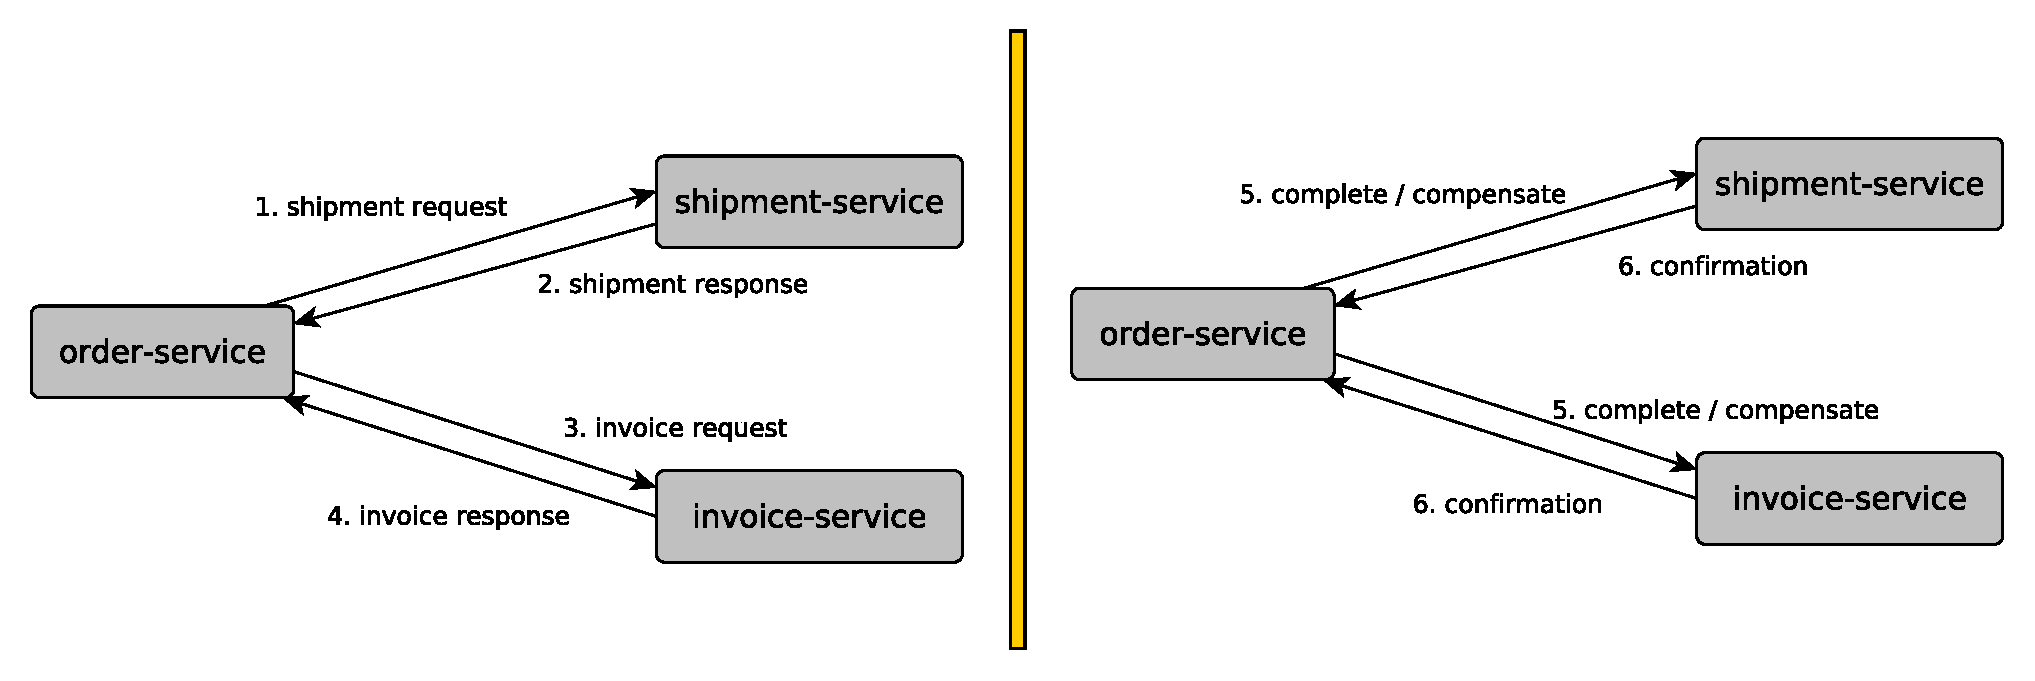
\includegraphics[height=40mm]{images/sagaModel.pdf}
    \end{center}
    \caption{The saga model}
\end{figure}

Every application is able to demonstrate three testing scenarios: the valid pass, the shipment failure and the invoice failure. In the valid scenario after the order is requested, the saga propagation invokes requests for the shipment and the invoice. If the connection between services is stable, both participants successfully return a stub answer and the order is completed. 

As most of the applied platforms invoke participants in the synchronous way, we distinguish separated member failures of the shipment or invoice. The shipment failure simulates the termination of saga without the full request coverage. This means that the compensations are distributed to all services including the \texttt{invoice-service} which has not received the work request for the order being processed yet. The scenario demonstrates the need of microservices to be able to react to the requests which are not associated with any saga which means actively keeping track of the sagas being currently executed. 

The invoice failure scenario on the other hand validates that the saga compensations are executed on all participating services as the shipment is already expected to be completed. Generally, the saga pattern assumes that the compensations of the participants are called in the reverse order of the invocations because of the possible dependencies between them.

To initiate the failures scenarios in examples both \texttt{shipment-service} and \texttt{invoice-service} are equipped with injected failure conditions. To invoke the failure the quickstarts expect a product information containing a specialized product identification: \texttt{fail-shipment} or \texttt{fail-invoice} respectively. 

The graphical representation in form of the sequence diagrams for corresponding scenarios is available in the Appendix C.

\section{Axon service}

As it was stated in the previous chapter, the Axon framework is based upon the CQRS principles. Because of this nature, it would be difficult not to follow this pattern. The individual services contain separated aggregates\footnote{for the definition of aggregate please refer to the Appendix A} each processing its respective commands and producing various events. Any inter-service interaction is restricted to the use of the command and event buses.

\subsection{Platform}

Axon service is a Java Spring Boot \cite{spring_boot} microservices application. Each service is fully separated and independent Maven  project \cite{maven}. Every project is standalone runnable application (fat jar\footnote{Java Archive}) as the Spring Boot does not use any underlying platform to run microservices.

As a CQRS based quickstart, Axon service uses two different and separated communication channels to exchange information between services: the command bus and the event bus. By default, the Axon framework reduce both channels to one JVM\footnote{Java Virtual Machine} thus one microservice. Except from that, developers are also able to specify several specialized ways of the configuration to distribute messages between different services which is used in this Axon quickstart.

The quickstart uses a motion of the distributed command bus which is based upon a different approach then the one used in the traditional single JVM Axon applications. The distributed command bus forms a bridge between separated command bus implementations to transfer commands between different JVMs \cite{axon_framework_reference_guide}. Its main responsibility is the selection of the communication protocol and the choice of the target destination for each incoming command. 

Axon provides two options for connecting different services through the distributed command bus -- \texttt{JGroupsConnector} and \texttt{Spring Cloud Connector}. The one used in this quickstart is the Spring Cloud method. The underlying implementation is based on the Netflix Eureka Discovery and Eureka Server combination \cite{service_registration}. Each business service as part of its initialization registers itself with the service \texttt{registration-server} which function as the Eureka server. Axon is then able to redirect commands to the right service chosen by the value of parameters in the command class annotated by the \texttt{@TargetAggregateIdentifier} annotation.

For the distribution of the event bus Axon service uses an external messaging system based on the Spring AMQP\footnote{Advanced Message Queuing Protocol} protocol called RabbitMQ message broker \cite{rabbitmq}. The quickstart uses separated messaging queue for each business service and one separated queue for the \texttt{query-service} microservice which is subscribed to all of the processing events. Axon platform provides the direct support for the AMQP so no specific handling of the produced events is required -- Axon automatically distributes events to all connected queues.

It is worth mentioning that both the Spring Cloud and the RabbitMQ message broker are required external providers that need to be started before the deployment of the business services. Unfortunaly, by the time of this writing there is no way to distribute commands or events directly by the Axon platform.

\subsection{Spring Boot}

\subsection{Project structure}

The application is composed of five microservices -- the  \texttt{order-service}, the \texttt{shipment-service}, the \texttt{invoice-service}, the \texttt{query-service} and the \texttt{registration-server}. Furthermore it also contains a separated project \texttt{service-model} which serves as a support library for the other microservices.

As it was stated in the previous section \texttt{registration-server} microservice is a Spring Boot application which function as a Netflix Eureka server. Other business services act as clients for this server, therefore it is required that this service is initialized by the time they try to register.

The \texttt{order-service} project is a business microservice responsible for the saga handling. It contains the logic for the order request, the saga initiation and the saga compensation.

Both \texttt{shipment-service} and \texttt{invoice-service} are business services functioning only as the saga participants. Their only obligation is to provide their respective computations.

The \texttt{query-service} is a specific microservice included for the purposes of the CQRS pattern. It collects the information of the prepared orders, shipments and invoices and provides an external APIs for the querying of these resources. 

Finally, the \texttt{service-model} is a Kotlin and Java Maven application providing the core API for the commands and events used by various business services. This is required as all classes must match in order for particular handlers to be invoked. Furthermore, it also provides common utilities and the logging support. It is mandatory to include this project on the classpath of the every other service.

\subsection{Problems}

\newlinepar{Maintenance of the saga structure}

The one substantial problem the saga processing in Axon has is the missing structure of the internal life cycle of the saga. Axon only provides ways to indicate the start and the stop of the saga. The actual invocation of the participants, collecting of the responses and handling of the compensations is up to developer as the only way of communication with the saga is through events.

In this application the \texttt{OrderManagementSaga} contains two internal classes -- \texttt{OrderProcessing} and \texttt{OrderCompensationProcessing} which are responsible for keeping track of the saga execution and compensation respectively. As production ready sagas can be expected to run in a number of days, this can quickly become the bottleneck of the saga maintenance.

\newlinepar{Distribution of events to sagas}

Another encountered problem is that by the time of this writing Axon does not provide an easy method for the configuration of the different event bus for saga events than is the one that is used by default. The \texttt{@Saga} annotation is preconfigured with the value of the local event bus which is not allowed to be changed. The workaround is to manually register a custom saga manager which is not straightforward from the user perspective when the saga needs to be distributed through different JVMs.

\newlinepar{AMQP usage with sagas}

When the distributed event bus is processing events from an AMQP queue which the saga class is listening to, the framework does not deliver events correctly to the attached handlers. This may be caused by the incorrect configuration from the previous problem. The workaround used in the quickstart is to artificially wait 1000 milliseconds before delivering the event from the queue to the framework.

\newlinepar{CQRS restrictions}

As CQRS is a pattern that manages the domain formation of the application, Axon can place a hard requirements for the projects that do not follow the CQRS domain separation. Like it was already presented, sagas in Axon are only a specialized type of the event listener. The only way Axon produces events is trough an interaction with the aggregate instance - events are produced purely as a response to the received command. Therefore the use of Axon sagas in not CQRS environment may be too restrictive for an implementation.

\section{Eventuate service}

Similarly to Axon, Eventuate service is also based on the event sourcing and the CQRS pattern. For this reason, the business execution is managed in the aggregates which correspond to the respective microservices projects. The communication is as a result restricted to the command processing and the event appliance.

This quickstart represents the pure CQRS approach to the saga processing. This means that the whole saga implementation is created by the developer using the platform only for the event and command distribution. For this reason, the Eventuate service is more complex than any other quickstart but for the example purposes, it distinctively demonstrates how sophisticated is the saga administration provided by all remaining platforms.

\subsection{Platform}
\label{sec:eventuate-platform}

Eventuate service is a microservices application consisting of a set of Spring Boot \cite{spring_boot} business services, one backing module and a number of support services provided by the Eventuate platform. In this section, I will focus on the Eventuate platform and the services it provides, the business part of the application is described in the following section.

This quickstart is established as a Eventuate Local version of the platform. This means that it uses underlying SQL database for the event persistence and the Kafka streaming platform for the event distribution. Eventuate Local provides five services used by the quickstart that are managed by the platform, namely Apache Zookeeper, Apache Kafka, MySQL database, the change data capture component and the Eventuate console service. The example employs these services as a Docker images included in the provided docker-compose configuration.

\newlinepar{Apache Zookeeper service}

Apache Zookeeper is an open-source project which enables highly reliable distributed coordination \cite{apache_zookeeper}. It maintains a centralized service which supervise various functionalities like handling of the configuration information, synchronization, naming or grouping. The Eventuate Local platform provides its own Docker image tagged as \texttt{eventuateio/eventuateio-local-zookeeper}.

\newlinepar{Apache Kafka service}

The Apache Kafka streaming platform is the service which is responsible for the administration of subscription and publishing mechanisms controlling the event processing for the business microservices. As it is based on the Streams API it allows the platform to react to events in real time. Eventuate manipulates Kafka as the notification service for the event propagation. Eventuate ships its own Kafka version in the \texttt{eventuateio/eventuateio-local-kafka} docker image.

\newlinepar{MySQL database service}

The SQL database used in this application for the event persistence is the MySQL open-source database which is currently the only database supported by the platform. The Eventuate Local maintains two tables -- \texttt{EVENTS} and \texttt{ENTITIES}. This database serves also as a transaction log maintained as a mean for the event sourcing. The containerized version is located under \texttt{eventuateio/eventuateio-local-mysql} tag.

\newlinepar{CDC service}

This service represents the change data capture (CDC) component. The CDC service has two main responsibilities -- it follows the transaction log and it publishes each event which is inserted into the \texttt{EVENTS} table to the Kafka topic that corresponds to the aggregate for which the event is intended. Eventutate Local supports two options of the execution of the CDC -- internally in each business service or as a standalone application. This quickstart applies the Eventuate CDC service \texttt{eventuateio/eventuateio-local-cdc-service} as a standalone Docker container.

\newlinepar{Eventuate console}

The last support service is the \texttt{consoleserver}. It provides a simple interface for accessing the information about created aggregate types and the event log. The supplied Docker container image is the \texttt{eventuateio/eventuateio-local-console}.

\subsection{Docker}

Docker is an open source container platform designed to make it easier to build, secure and manage the widest array of application from development to production both on premises and in the cloud \cite{docker}. Docker containers allow applications to run on top of the kernel services provided by the hosting system which considerably effects the application performance. However, it still builds containers on top of the generalized interface which warrants straightforward portability between different machines.

A container image is a lightweight, stand-alone, executable package of a piece of software that includes everything needed to run it -- code, runtime, system tools, libraries or settings \cite{docker}. All docker containers that run on the same machine share the kernel services of the host. The images are build on the concept of layers. The layer provides an abstraction to share common filesystems, configuration and other data that can be reused by several docker containers.

Containers isolate applications from the operating system their running on and also provide the separation from other docker containers running concurrently on the same computer. Instead of virtual machines which provide similar functionality, Docker virtualizes the operating system not the hardware. Docker provides abstraction at the application level.

Docker as a tool is targeted for simple utilization. It provides an unified environment for both developers and administrators supporting the DevOps (development and operations) practices. Particularly, developers profit from portable code that is able to run on any operating platform supporting Docker, while operations gain visibility and management services from comprehensive control panel covering all containerized applications.

\subsection{Project structure}

This section describes the set of services composing the business side of the application. This set contains four services that cover the saga execution and data processing (\texttt{order-service}, \texttt{shipment-service}, \texttt{invoice-service} and \texttt{query-service}), one service (\texttt{mongodb}) representing the persistent storage and one additional support module (\texttt{service-model}).

All of the business services are a Spring Boot applications based on the Gradle \cite{gradle} build system. Each microservice is represented as a independent module capable of being separately built and deployed. Even if Spring Boot projects can be executed directly from the command line as ordinary Java applications, this quickstart leverages the Docker approach of the Eventuate Local platform and containerize all of its services.

To connect to the Eventuate platform each service defines a set of environment variables. This information includes the connection and authentication details for the MySQL database, the CDC component and the connection URLs\footnote{Uniform Resource Locator} for the Kafka and the Zookeeper services. These variables are specified in the container specification for each individual business service in the \texttt{docker-compose.yml} file.

The actual saga execution is managed in the \texttt{order-service} microservice. The saga realization implementation is contained in three classes -- the \texttt{OrderSagaAggregate}, the \texttt{SagaEventSubscriber} and the \texttt{OrderSagaService}. The first class is an ordinary CQRS aggregate that handles the commands for the saga initialization and the participants outcomes. Conversely, the latter one is the event processor listening for the events produced by the aggregate which is basically a wrapper around the \texttt{OrderSagaService} - the class responsible for the remote REST calls to the other services and the command dispatching for the \texttt{OrderSagaAggregate}. The usage of the separated event listener is required because Eventuate does not allow aggregates to be declared as Spring components. The reason of this defect is described in more detail in the following section.

Except for the normal order API, the \texttt{order-service} also provides a management API for the participants to be able to share the information about their processing. This endpoints are hardcoded in the application which may not be acceptable for a production realization.

The \texttt{shipment-service} and the \texttt{invoice-service} both contain a simple aggregate together with its associated event listener which control the participant interaction with the saga. Each service also accommodate the REST endpoint for the saga request and its possible compensation.

Similarly to Axon service, the \texttt{service-model} project acts as a support library for other services. It contains a core API for each business service which needs to be shared and the utilization classes.

The last business microservice is the \texttt{query-service}. It performs as a response service providing the information about persisted orders, shipmetns and invoices. It contains an event listener for each designated microservice which in turn preserve the achieved information in the Mongo NoSQL database. This service also provides a simple Swagger interface to ease the user application interaction.

\subsection{Problems}

\newlinepar{Complexity}

As this project represents a plain CQRS based example it completely demonstrates the background process required for the saga execution. Therefore the complexity of this quickstart may appear more critical than in other projects as the background saga execution often contains many optimizations.

The first complexity problem is that the project contains a great number of the command and event classes. This is required as aggregate classes are only able to consume commands and produce events. For that reason,  the communication between components often demands a few additional steps.

The full saga administration is handled by the project from the very beginning. That covers the support of starting, stopping and following the saga execution as well as saga compensations. The restrictions placed by the CQRS pattern furthermore put additional requirements on the saga processing which may not be demanded by other frameworks. Before the Eventuate Tram framework, the Eventuate platform did not provide any saga support.

This quickstart uses the REST architectural style for the remote communication between services. Even if all of microservices are connected to the same MySQL database, they cannot directly propagate commands between each other. This is due to the way Eventuate dispatches commands through the aggregate repository. The aggregate repository represents the database table that is restricted to one aggregate and consequently, it needs to be injected by the platform. For this reason, it needs to declare the target aggregate class and the command type. The sharing of the aggregate class may be very restrictive, especially for microservices applications.

\newlinepar{Aggregate instantiation}

The Eventuate framework creates the instances of the aggregate classes by a call to the default constructor. This effectively prohibits the use of aggregate instance managed by the underlying server container. 

For this reason, each aggregate in this project is separated into two classes -- the actual aggregate responsible for the command processing and the event subscriber instance managing the incoming events. The  aggregate class is required to extend the \texttt{ReflectiveMutableCommand\\ProcessingAggregate} specifying the type of the command interface which allows the classpath instantiation. The event listener is defined by the \texttt{@EventSubscriber} annotation which permits it to be constructed as a Spring container component for the dependency injection employment. 

This restriction is seconded by the rule stating that each produced event from the aggregate's command processing method must also be applied by the different method of the same aggregate. This limitation exists because of the event sourcing feature providing the ability to replay already executed commands to reconstruct the aggregate's state in the case of failure. The aggregate then may contain unnecessary empty methods as the saga also requires the propagation of the information to different components (e. g. the REST controller).


\newlinepar{Event entity specification}

As well as the command type, Eventuate also requires the definition of the event type each aggregate is able to produce. The event class is defined as a value of the \texttt{entity} attribute of the \texttt{@EventEntity} annotation. This annotation is usually placed on the event interface which implementation represents produced events.

The problem rises when the events needs to be shared between several modules. This is a common requirement as the CQRS pattern requires the query domain to be separated. The event interfaces are therefore included in the common library module as the \texttt{service-model} used in this project. The hard coded information of the full name of the aggregate class used in the \texttt{@EventEntity} annotation then may become hard to maintain.

\newlinepar{Platform structure}

The platform structure places the obligation on each developed microservice to conduct with the connecting specification. This means that every service must provide linking information for the Eventuate platform services described in the previous section, namely MySql database, Apache Kafka, Apache Zookeeper and CDC component. This information is manually replicated in each service (restricted to system properties) and therefore predisposed to errors.

\hfill \break

In the end it is worth mentioning that as the Eventuate service is the pure CQRS saga example it has a few problems which has been reduced or removed in the later Eventuate Tram implementation that is in detail described in the following section. 

\section{LRA service}

The LRA service is the first example in contradiction with previous quickstarts as it does not restrict its services to any particular conventions. Individual services are connected through the exposed REST routes.

\subsection{Platform}

This quickstart is composed as a set of WildFly Swarm microservices applications. Every microservice is designed to be easily deployed to the OpenShift container application platform provided by Red Hat, Inc. Both of these platforms are in detail described in the following sections.

Each service uses the \texttt{fabric8-maven-plugin} for the build and the deployment to the OpenShift platform. This plugin provides a straightforward way of declaring the necessary description information the platform requires to orchestrate the service according to the user demands. This project applies the source to image (S2I) toolkit that builds imminent Docker images which can by immediately deployed to the OpenShift. 

As it was already presented in the previous chapter Narayana's long running actions are not composed as a platform, rather as a standalone library. This project builds upon the use of the Narayana LRA coordinator which is same as the other services constructed as a WildFly Swarm microservice called \texttt{lra-coordinator}. 

The traditional requirements placed on the microservices applications are handled by the OpenShift platform. That for instance covers service discovery and location transparency, monitoring, logging, resiliency and health checks (failure discovery). 

\subsection{WildFly Swarm}

WildFly Swarm is the Red Hat microservices initiative designed to enable deconstructing the WildFly application server and pasting just enough of it back together with the application to create a self-contained executable jar \cite{gupta_2018}. 

The traditional Java EE\footnote{Enterprise Edition} approach follows the development of the application and its successive deployment to the application server which includes necessary dependencies which the application requires to run. On the other hand, Wildfly Swarm creates a fat Java archive which packages all needed dependencies inside itself. This emulates the packaging of only requisite parts of the application server. The result jar is a standalone runnable Java application which can be executed by the \texttt{java -jar} command. It also provides Maven and Gradle plugins to ease the development of Swarm applications.

The default fat jar (also called the uberjar) contains the user application and the needed parts of the WildFly server. Swarm also supports the packaging of the necessary server parts separately from the application. This method is know as the hollow jar and is particularly useful in the containerized environment as the server may be placed in the lower layers that do not require frequent rebuilds.

The individual server parts are being delivered in the packages named fractions. The fraction represents a precise selection of capabilities that can be included in the application. It may denote the exact WildFly subsystem as JAX-RS\footnote{Java API for RESTful Web Services} or CDI\footnote{Context and Dependency Injection}, or a more sophisticated set of facilities to provide some additional functionality like RHSSO\footnote{Red Hat Single Sign-On}.

\subsection{OpenShift platform}

Red Hat OpenShift is an open source container application platform that  brings Docker and Kubernetes to the enterprise \cite{openshift} generally build on top of the Red Hat Enterprise Linux. It provides the deployment, management and monitoring of the containerized software. OpenShift provides automation in the cloud environment that enables simple development workflow including easy provisioning, building and deployment of enterprise applications allowing faster delivery to end customers.

The platform provides extensive set of features like self-service maintenance, polyglot (language independent) application support, container-based environment and the automation of application builds, scaling and health management. It can also administer persistence capabilities, the application centric networking and multiple interaction models, e. g. command line tools or the web console.

OpenShift is being developed in several variants. The upstream community project is OpenShift Origin which is a distribution of Kubernetes optimized for continuous application development and multi-tenant deployment \cite{openshift}. On top of the Kubernetes platform, Origin provides the developer and operations centric tooling, security, logging or pipelining and many other capabilities. Origin is also available as the all in one virtual machine called Minishift which utilizes a local single-node OpenShift cluster. 

The second alternative is the OpenShift Online. Currently distributed in version 3, it serves as a Red Hat public cloud application development and hosting service. OpenShift Online provides an integrated environment that allows developers to focus on the application development instead of its management through the set of facilities like source-to-image builds eliminating the Dockerfiles creation, one click deployments through git hooks, automatic scaling according to the traffic and integration with the Eclipse IDE\footnote{Integrated Development Environment}.

OpenShift Dedicated offers a managed private cluster which can be hosted on the public cloud like Amazon Web Services or Google Cloud platform. It provides OpenShift services as an isolated platform that aims for the simple and faster transition of user applications to the container based and native cloud environments.

The last OpenShift variant it the OpenShift.io. It provides an open online end-to-end development environment for planning, creating and deploying hybrid cloud services \cite{openshift_io}. It supports an integrated approach to DevOps, including tools as one-click container management, machine learning system and integration of many projects like fabric8 or Eclipse Che.

\subsection{Kubernetes}

Kubernetes is an open source project providing automation, scaling and management of containerized applications \cite{kubernetes}. It groups the application containers into logical units for easier management and discovery.

The features of Kubernetes include the service discovery, load balancing, automatic container placement or the self-healing for the automated failure recovery and rollbacks. It also manages the storage orchestration, scaling of containers, secrets, container configuration and batch capabilities.

Kubernetes platform is suitable and portable to any cloud environment involving public, private, hybrid clouds and multi-cloud. It allows application containers to be run in the clusters of physical or virtual machines. Kubernetes is not a traditional PaaS (Platform as a Service) solution but it provides platform that many PaaS systems build upon, e. g. OpenShift or Deis.

\subsection{Project structure}

This project consists of five WildFly Swarm microservices and one support module. Each service is designed and configured with the \texttt{fabric8-maven-plugin} providing simple deployment to the OpenShift platform. Additionally, services contain a customized Dockerfile specifying environment properties and the target Swarm uberjar file which is used for the source-to-image (S2I) builds in OpenShift.

The support library project is called the \texttt{service-model}. This module is rosponsible for the definition of the LRA information, the specification of the exchanged JSON data formats, the characterization of the communication model used in other services and the administration of common utilities.

The \texttt{LRADefinition} class denotes the JSON format of the LRA representation. It presents a simplified version of the LRA capabilities for the example purposes. The definition includes only required attributes -- the name of the LRA, a list of individual actions that form the LRA and the unspecified object containing the user defined information associated with the LRA. The example LRA definition JSON format is available in the figure 6.3.

\begin{figure}
    \begin{center}
        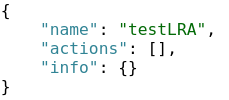
\includegraphics[height=30mm]{images/LRADefinition.png}
    \end{center}
    \caption{LRA definition example JSON}
\end{figure}

The individual actions that compose the LRA are incident to the pattern services in this quickstart use for the communication. The information exchange is based upon the REST architectural style which expects that services adhere to predefined endpoint rules. 

The action definition consists of the name, the action type and the service for which the invocation is intended. The \texttt{service-model} project contains both \texttt{ActionType} and \texttt{Service} enumerations that denote possible values. The example action JSON is included in the figure 6.4.

\begin{figure}
    \begin{center}
        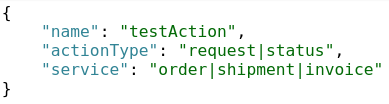
\includegraphics[height=30mm]{images/actionJSON.png}
    \end{center}
    \caption{Action example JSON}
\end{figure}

The actual deployable microservices project consists of five services -- \texttt{api-gateway}, \texttt{order-service}, \texttt{shipment-service}, \texttt{invoice-service} and \texttt{lra-coordinator}. Every service is configured with the addresses of other services as they reflect the OpenShift/Kubernetes application names. All of exposed APIs are defined in the Appendix B.

The services that provide the LRA execution capabilities are the \texttt{order-service}, the \texttt{shipment-service} and the \texttt{invoice-service}. Every one of these services provides a simple computation that contributes to the LRA realization. Additionally, \texttt{order-service} also provides a user invocation endpoint that can initiate the LRA. As all three services eventually subscribe to the LRA when they are called, they all provide REST endpoints annotated by the LRA annotations for the completion and compensation invocations. Each service is configured with an instance of H2 SQL database for the data persistence.

The \texttt{lra-coordinator} project is provided by the Narayana framework. Although the LRA specification does not require the application of the REST architectural style, the \texttt{lra-coordinator} operates a set of REST endpoints maintaining the starting and managing of the LRA, gathering the information about active and recovering LRAs, the management of the nested LRAs and the ability of participants to join or leave the LRA. Narayana distributes this project already as a WildFly Swarm binary but this quickstart, for the investigation purposes, builds it still as a part of the S2I deployment.

Even if the \texttt{lra-coordinator} presents the REST endpoints for the LRA management, this quickstart invokes the coordinator by the client module provided by Narayana. The \texttt{lra-client} dependency provides the \texttt{LRAClient} class that is configured with the coordinator location and serves as a proxy separating the user from the actual REST invocations. This class is defined as a CDI bean to enable the dependency injection across the project. \texttt{LRAClient} is able to also control the whole LRA lifecycle but the prefered method is to use the annotations present in the \texttt{io.narayana.lra.annotation} package.

The last service is the \texttt{api-gateway}. This module functions as an interface that makes the LRA execution transparent for the invoking services. The current state of the Narayana handling of LRA calls will be described in the following section.

The \texttt{api-gateway} uses the LRA and action definition classes from the \texttt{service-module} to handle the LRA processing on the behalf of the initiating user. It exposes a REST interface that consumes the LRA definition JSON.

The actual LRA execution is managed in the \texttt{LRAExecutor} class. This class provides one public method \texttt{processLRA(LRADefinition lraDefinition, String baseUri) : LRAResult} that is responsible for starting and performing of the LRA, collecting the participants results and closing or compensating of the LRA. The \texttt{baseUri} attribute is present because the \texttt{api-gateway} service subscribes to the started LRA as the initiator.

As this module was designed for this particular LRA scenario, it is configured to execute the LRA actions (shipment and invoice requests) independently and in parallel. It collects the result of each action and eventually closes or cancels the LRA with methods provided by the \texttt{LRAClient}. Certainly, this is an area which could be in a more general execution module further extended with e.g. sequential configuration or LRA nesting.

\subsection{Problems}

The Narayana Long running actions a very nice development model for the microservices applications. As it aims for the compatibility with the MicroProfile specification, it does not restrict services to essentially any particular implementation restrictions. Even if the MicroProfile is restricted on REST invocations, Narayana LRA specification does not require the usage this architectural style for the communication with the coordinator. However, the only implementation that is currently available is based on REST, but in can be efficiently extended to other communication protocols in the future.

The only problem that may occur is that currently, the LRA framework provides only coordination and management capabilities, it does not handle the saga structuring and execution. This may be controversial as any of the previous frameworks did not exposed this functionality neither. The idea was introduced by the Eventuate Tram framework which is described in the following section. This concern may be troublesome for the enterprise ready reactive microservices, as it may place restrictions on their availability under substantial traffic. 

In the LRA service is this problem addressed by the \texttt{api-gateway} service which functions as a proxy for the \texttt{lra-coordinator} that handles the saga execution. This approach does not effect the Narayana LRA management. The only change from the traditional processing is that series of LRA actions are performed by the \texttt{api-gateway} instead of the initiating service. This allows the service to be immediately available for the subsequent user requests and to scale the LRA processing independently from the services that utilize the coordination.

\section{Eventuate Sagas}

The Eventuate Sagas quickstart is based on the new Eventuate Tram framework which is still, by the time of this writing, under pre-release development. This framework provides several solution to problems with saga management that are present in the Eventuate platform.

\subsection{Platform}

Similarly to the full Eventuate distribution, the Eventuate Tram establishes four services that form the Tram platform: Apache Zookeeper, Apache Kafka, MySQL database and CDC component. The fifth Console service is not present as the platform does not provide this functionality by the time of this writing. As all mentioned services represent the same functionality as they are responsible for in the full Eventuate platform, the individual descriptions of each service is defined in detail in the section \ref{sec:eventuate-platform}.  

All services are deployed by the \texttt{docker-compose} configuration distributed with the framework. This setup is based on the same Eventuate docker images for \texttt{zookeeper} and \texttt{kafka} services, and with \texttt{mysql} and \texttt{cdcservice} redefined by Tram.

\subsection{Project structure}

As Eventuate Tram does not restrict its services to the CQRS pattern, this project, in contrast to Eventutate service, contains only three business microservices and one support module. Every service is configured in the similar way as for the full platform containing the references and authentication details for the MySQL database, Kafka framework and Apache Zookeeper service. The quickstart is distributed with the predefined \texttt{docker-compose} configuration file that enables one command start up of all services.

The last service which is not required for the saga execution and handling is the \texttt{mongodb} NoSQL server. This service is present only for the demonstration purposes to allow the data retrieval on individual business services.

The first microservice \texttt{order-service} is responsible for the order requests and saga processing. It also provides the ability to query persisted orders from the remote Mongo database.

The most important element in the \texttt{order-service} is the saga definition that is located in the \texttt{OrderSaga} class. This definition uses the declarative approach with the fluent API to denote the saga in steps of execution. Every step declares a handler method to be invoked when the step is reached by a reference to private methods in this class.

The step provides an ability to advance the saga execution in three ways -- by invoking of the local function, by a call to the remote participant or by the definition of the compensation method for the saga. Furthermore, the participant is able to define individual actions that comprise its engagement in the saga, the compensation handler and several reply handlers that are distinguished by the data object class that is received in the reply. This definition provides a simple in one place saga specification which is suitable for easier maintenance and distribution. This declarative approach provides many advantages that will be detailed in the following chapter.

The last two business services that contribute to the saga execution are \texttt{shipment-service} and \texttt{invoice-service}. Both of these microservices define several command handler methods associated with the channel that is dedicated to the service. 

The channel is a main communication mechanism used in Eventuate Tram. It is denoted by a string name that needs to be specified in the command message as a target destination. The definition of channel associates commands that it is able to receive with command handling methods that are invoked when the corresponding commands are delivered. The command handler returns a \texttt{Message} object identifying the outcome of the invocation. The failure outcome of any participant will immediately result in the saga compensation.

Both services are also connected to the Mongo database server in order to provide the browsing of the created shipments or invoices respectively.

In conclusion, Tram remarkably simplified the Eventuate platform for the usage of sagas. Most importantly, it introduced a simple fluent API for the saga definition and the loss of CQRS restrictions. Altogether, Tram platform makes a suitable saga solution for microservices based environment.

\subsection{Problems}

\newlinepar{Destination identification}

The destination channels in Tram are distinguished by a simple string which may cause problems in the case of name conflicts. Currently, the choice of the handler to be invoked depends on two resources -- the name of the channel and the command dispatcher id. When both strings match the same destination even in different services, the platform delivers the commands between handlers in random fashion which may become a complex issue in larger projects.

\newlinepar{Command handlers}

Handler methods that are referenced in the definition are restricted to the communication model provided by the platform. This allows a single command to be sent to the required destination. Unfortunately, platform does not allow the saga to perform any other operation without the participant invocation which may lead to unnecessary empty commands and channels declarations. 

Similarly, the saga may need to interact with the same participant in several different commands. This may cause problems with definitions of compensation and reply handlers as the developer needs to mind the logical grouping of participant invocations.

\clearpage
\chapter{LRA execution extension}

\clearpage
\chapter{Conclusion}



\makeatletter\thesis@blocks@clear\makeatother
\phantomsection %% Print the index and insert it into the
\addcontentsline{toc}{chapter}{Bibliography} %% table of contents.
\printindex

\bibliographystyle{myIEEEtran}
\bibliography{IEEEabrv,references}

\appendix %% Start the appendices.

\chapter{The Command Query Responsibility Segregation pattern}

CQRS

\chapter{The example applications public APIs}
\label{sec:appendixAPI}

\section{Axon service}

\textbf{Order service}

\begin{minted}{python}
        POST /api/order
\end{minted}

\noindent
\textbf{Query service}

\begin{minted}{python}
        GET /api/orders
        GET /api/order/{order_id}
        GET /api/shipments
        GET /api/shipment/{shipment_id}
        GET /api/invoices
        GET /api/invoice/{invoice_id}
\end{minted}

\section{Eventuate service}

\textbf{Order service}

\begin{minted}{python}
        POST /api/order
        POST /management/shipment
        POST /management/shipment/fail
        POST /management/shipment/compensation
        POST /management/invoice
        POST /management/invoice/fail
        POST /management/invoice/compensation
\end{minted}

\noindent
\textbf{Shipment service}

\begin{minted}{python}
        POST /api/request
        POST /api/compensate
\end{minted}

\noindent
\textbf{Invoice service}

\begin{minted}{python}
        POST /api/request
        POST /api/compensate
\end{minted}

\noindent
\textbf{Query service}

\begin{minted}{python}
        GET /api/orders
        GET /api/order/{order_id}
        GET /api/shipments
        GET /api/shipment/{shipment_id}
        GET /api/invoices
        GET /api/invoice/{invoice_id}
\end{minted}

\section{LRA service}

\textbf{Order service}

\begin{minted}{python}
        POST /api/order
        GET  /api/health
\end{minted}

\noindent
\textbf{Shipment service}

\begin{minted}{python}
        POST /api/request
        PUT  /api/complete
        PUT  /api/compensate
        GET  /api/health
\end{minted}

\noindent
\textbf{Invoice service}

\begin{minted}{python}
        POST /api/request
        PUT  /api/complete
        PUT  /api/compensate
        GET  /api/health
\end{minted}

\noindent
\textbf{LRA coordinator}

\begin{minted}{python}
        GET  /lra-coordinator
        GET  /lra-coordinator/{LraId}
        GET  /lra-coordinator/status/{LraId}
        POST /lra-coordinator/start
        PUT  /lra-coordinator/{LraId}/renew
        GET  /lra-coordinator/{NestedLraId}/status
        PUT  /lra-coordinator/{NestedLraId}/complete
        PUT  /lra-coordinator/{NestedLraId}/compensate
        PUT  /lra-coordinator/{NestedLraId}/forget
        PUT  /lra-coordinator/{LraId}/close
        PUT  /lra-coordinator/{LraId}/cancel
        PUT  /lra-coordinator/{LraId}
        PUT  /lra-coordinator/{LraId}/remove
        GET  /api/health
        GET  /lra-recovery-coordinator/{LRAId}/{RecCoordId}
        PUT  /lra-recovery-coordinator/{LRAId}/{RecCoordId}
        GET  /lra-recovery-coordinator/recovery
\end{minted}

\noindent
\textbf{API gateway}

\begin{minted}{python}
        PUT  /api/complete
        PUT  /api/compensate
        GET  /api/health
        POST /api/lra
\end{minted}


\section{Eventuate Tram}

\textbf{Order service}

\begin{minted}{python}
        POST /api/order
        GET  /api/orders
        GET  /api/order/{orderId}
\end{minted}

\noindent
\textbf{Shipment service}

\begin{minted}{python}
        GET /api/shipments
        GET /api/shipment/{shipmentId}
\end{minted}

\noindent
\textbf{Invoice service}

\begin{minted}{python}
        GET /api/invoices
        GET /api/invoice/{invoiceId}
\end{minted}


\chapter{JTA}
\label{sec:appendix-JTA}

\noindent
\textbf{javax.transaction.UserTransaction}

\begin{minted}{java}
    void begin();
    
    void commit();
    
    void rollback();
    
    void setRollbackOnly();
    
    int getStatus();
    
    void setTransactionTimeout(int seconds);
\end{minted}

\hfill \break

\noindent
\textbf{javax.transaction.Status}

\begin{minted}{java}

    STATUS_ACTIVE = 0;

    STATUS_MARKED_ROLLBACK = 1;

    STATUS_PREPARED = 2;

    STATUS_COMMITTED = 3;

    STATUS_ROLLEDBACK = 4;

    STATUS_UNKNOWN = 5;

    STATUS_NO_TRANSACTION = 6;

    STATUS_PREPARING = 7;

    STATUS_COMMITTING = 8;

    STATUS_ROLLING_BACK = 9;
\end{minted}

\noindent
\textbf{javax.transaction.TransactionManager}

\begin{minted}{java}
    void begin();
    
    void commit();
    
    void rollback();
    
    void setRollbackOnly();
    
    int getStatus();
    
    Transaction getTransaction();
    
    void setTransactionTimeout(int seconds);
    
    Transaction suspend();
    
    void resume(Transaction tobj);
\end{minted}


\chapter{The saga scenarios}


\end{document}
